\documentclass[tikz,border=5pt]{standalone}
\usepackage[utf8]{inputenc}
\usepackage[T1]{fontenc}
\usepackage{lmodern,amsmath,amssymb}
\usepackage[american]{circuitikz}
\usepackage{pgfplots}
\pgfplotsset{compat=1.18}
\usetikzlibrary{circuits.logic.US,positioning,calc,arrows.meta,patterns,shapes.geometric}
\definecolor{Primary}{HTML}{1F77B4}
\begin{document}
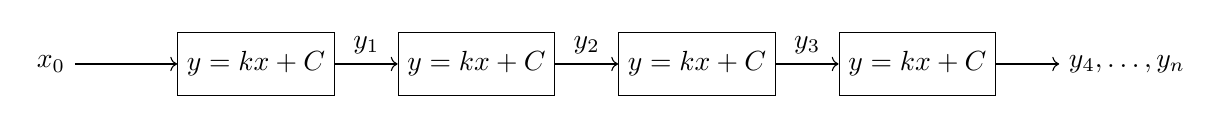
\begin{tikzpicture}\foreach\i in{1,...,4}{\node[draw,minimum width=1.5cm,minimum height=.8cm](b\i)at(2.8*\i,0){$y=kx+C$};}\draw[->](.5,0)node[left]{$x_0$}--(b1.west);\foreach\i/\j in{1/2,2/3,3/4}{\draw[->](b\i.east)--node[above]{$y_\i$}(b\j.west);}\draw[->](b4.east)--(13,0)node[right]{$y_4,\ldots,y_n$};\end{tikzpicture}
\end{document}
